\documentclass[fleqn,letterpaper,12pt,printwatermark=false]{memoir}
% memoir commands to define the text block geometry
\setulmarginsandblock{0.5in}{*}{*}
\setlrmarginsandblock{0.5in}{*}{*}
% put "extra" vertical space at the bottom of a page
\raggedbottom 

\usepackage{amsmath}
\usepackage{etoolbox} % for \ifblank etc
\usepackage{xparse} % for NewDocumentCommand et al.
\usepackage{enumitem}
\usepackage{transparent} % for \transparent, which I use in the watermark
\usepackage[slantedGreek]{mathpazo} \usepackage{helvet} % use Palatino et al.
\usepackage{booktabs} % prettier tables

\usepackage[]{xwatermark}
\newwatermark*[
    allpages,
    color=red!30,angle=45,
    scale=4,
    xpos=-10, ypos=0
]{%
    \transparent{0.4}dhasan example%
}

\usepackage{dashundergaps} % for \gap
\dashundergapssetup{
    teacher-mode=true, % set to true to show answers 
    gap-format=underline,
    teacher-gap-format=underline,
    gap-font={\sffamily},
    gap-numbers=true,
    gap-widen=true,
    gap-extend-percent=150, % note: making this too big might create errors
    gap-number-format=\,\textsuperscript{\normalfont(\thegapnumber)},
}

\usepackage{tcolorbox}
\tcbuselibrary{skins}
\tcbuselibrary{raster}

\usepackage{graphicx}
\graphicspath{ {../images/} }
\begin{document}

\newcommand{\myClassName}{Pre-AP Algebra 2}
\newcommand{\myUnitNumber}{1}
\newcommand{\myUnitTitle}{Introduction to Functions}
\newcommand{\myLessonNumber}{7}
\newcommand{\myLessonTitle}{Graphing Linear Equations}


\copypagestyle{myPagestyle}{empty}


\newcommand{\myFooterSize}{\footnotesize}
\makeoddfoot{myPagestyle}{{}}{\myFooterSize{\thepage{}~of~\pageref*{xwmlastpage}}}{\myFooterSize\thetitle}
\makeevenfoot{myPagestyle}{{}}{\myFooterSize{\thepage{}~of~\pageref*{xwmlastpage}}}{\myFooterSize\thetitle}

%
% A command to change the appearance of the cognitive verb 
% in the objectives.
%
\newcommand{\myCognitiveVerb}[1]{\textcolor{blue}{\textbf{#1}}}

%
% Terminology explanation:
%
% "unit" refers to the Algebra 2 unit being taught.
% "section" refers to the section within the unit being taught.
% "heading" refers to the headings in this document (Objectives, Example, ...)
%
\NewDocumentCommand{\myUnitSectionNumberFont}{}{\sffamily\bfseries\HUGE}
\NewDocumentCommand{\myUnitNameFont}{}{\sffamily\large}
\NewDocumentCommand{\mySectionNameFont}{}{\sffamily\bfseries\huge}
\NewDocumentCommand{\myHeadingFont}{}{\sffamily\bfseries\Large}


%
% #1 is the fill-in text
%
\NewDocumentCommand{\myFillInBlank}{m}{%
    \,%
    \gap[u]{#1}%
    \,%
}


% Definition for the LESSON HEADER + OBJECTIVES
%
% #1 : optional unit name
% #2 : optional unit/section number
% #3 : mandatory title
%
\NewDocumentEnvironment{myNotesHeader}{oom}{
    \title{#3}
    \begin{flushleft}
        \IfValueT{#2}{{\myUnitSectionNumberFont#2}}
        \hfill\;\;
        \begin{minipage}[b]{0.75\textwidth}
            \begin{flushright}
                \IfValueT{#1}{
                    {\myUnitNameFont#1}\\ \vspace{0.75em}
                }
                {\mySectionNameFont#3}
            \end{flushright}
        \end{minipage}
        \hrule
    \end{flushleft}
    \noindent{\myHeadingFont Objectives:}
    \begin{enumerate}[label=\arabic*)]
}{
    \end{enumerate}
}


% Definitions related to the VOCABULARY TABLE
%
\newenvironment{myVocabulary}{
    {\noindent{\myHeadingFont Vocabulary:}}\vspace{1em}

    \begin{tabular}{ll}
        \toprule
            \emph{word} & \emph{meaning} \\ 
        \midrule
}{
    \bottomrule
    \end{tabular}
    \vspace{1em}
}

\newcommand{\myVocabularyWord}[2]{%
{\textcolor{blue}{\textbf{#1}}} & #2 \\
}


% Definitions related to an INTRODUCTION
%
\newenvironment{myIntroduction}{
    {\noindent{\myHeadingFont Introduction:}}\vspace{1em}

    \setlength{\leftskip}{3cm}
}{
    \setlength{\leftskip}{0pt}
}


% Definition related to KEY CONCEPTS
%
% #1 : the key concept (which appears as a tcolorbox title)
%
\NewDocumentEnvironment{myKeyConcepts}{ O{Key Concepts:} }{
    \begin{tcolorbox}[
        title=#1, fonttitle=\myHeadingFont,
        coltitle=black, 
        colbacktitle=black!25!yellow, 
        colframe=black!50!yellow,
        colback=white!70!yellow,
        boxrule=2pt, 
        ]
}{
    \end{tcolorbox}
}


% Definition related to EXAMPLES
%
% #1 Optional example number 
% #2 A statement of the example problem.
% #3 How much empty vertical space to leave for the example box.
%
\NewDocumentCommand{\myExample}{omm}{%
    \begin{tcolorbox}[
        enhanced,
        sharp corners, 
        colback=white,
        boxrule=0pt,
        borderline={0.5pt}{0pt}{black,dashed},
        ]
        {\myHeadingFont Example\IfValueT{#1}{{ #1}}:}
        #2
        \tcblower
        \vspace{#3}
    \end{tcolorbox}
}

% Definitions related to PROBLEMS

% A counter to number the problems in the guided notes.
\newcounter{MyProblemCounter}
\setcounter{MyProblemCounter}{1}
\newcommand{\useMyProblemCounter}{\theMyProblemCounter\stepcounter{MyProblemCounter}}

% an environment for two adjacent problems
%
% #1 : directions for all the problems
% #2 : vertical height of the problem boxes
% #3 : details for problem 1
% #4 : details for problem 2
%
\newenvironment{myProblems2}[4]{%
    \noindent
    {\myHeadingFont Practice:}\hspace{0.5em}#1\nopagebreak%
    \begin{tcbraster}[%
        raster equal height,%
        raster columns=2,%
        raster column skip=0.5mm,%
        raster row skip=0.5mm,%
        raster every box/.style={%
            enhanced,%
            sharp corners,%
            colback=white,%
            coltitle=black, colbacktitle=black!10!white,%
            boxrule=0pt, borderline={0.5pt}{0pt}{black},%
            title={\texttt\useMyProblemCounter},%
            },%
        ]%
        \begin{tcolorbox}[attach boxed title to top left]
            #3
            \tcblower\vspace{#2}
        \end{tcolorbox}
        \begin{tcolorbox}[attach boxed title to top right]
            #4
            \tcblower
        \end{tcolorbox}%
}{%
    \end{tcbraster}
}

% an environment for 4 adjacent problems
%
% #1 : directions for all the problems
% #2 : vertical height of the problem boxes
% #3 : details for problem 1
% #4 : details for problem 2
% #5 : details for problem 3
% #6 : details for problem 4
%
\newenvironment{myProblems4}[6]{%
    \noindent
    \textbf{\myHeadingFont Practice:}\hspace{0.5em}#1\nopagebreak%
    \begin{tcbraster}[%
        raster equal height,%
        raster columns=2,%
        raster column skip=0.5mm,%
        raster row skip=0.5mm,%
        raster every box/.style={%
            enhanced,%
            sharp corners,%
            colback=white,%
            coltitle=black, colbacktitle=black!10!white,%
            boxrule=0pt, borderline={0.5pt}{0pt}{black},%
            title={\texttt\useMyProblemCounter},%
            },%
        ]%
        \begin{tcolorbox}[attach boxed title to top left]
            #3
            \tcblower\vspace{#2}
        \end{tcolorbox}
        \begin{tcolorbox}[attach boxed title to top right]
            #4
            \tcblower
        \end{tcolorbox}%
        \begin{tcolorbox}[attach boxed title to bottom left]
            #5
            \tcblower
        \end{tcolorbox}%
        \begin{tcolorbox}[attach boxed title to bottom right]
            #6
            \tcblower
        \end{tcolorbox}%
}{%
    \end{tcbraster}
}
\pagestyle{myPagestyle}

\checkandfixthelayout
\setlist{labelindent=\parindent,leftmargin=*,itemsep=0.025em,label=$\circ$}

% ---------------------HEADER------------------------------
\begin{myNotesHeader}
    \item \myCognitiveVerb{sketch} the graph of a line from its intercepts
    \item \myCognitiveVerb{sketch} the graph of a linear equation
\end{myNotesHeader}

\begin{myVocabulary}
    \myVocabularyWord{intercepts}
        {
            the points where a curve (line) crosses the $x$ and $y$ axes
        }
        \myVocabularyWord{sketch}
        {
            draw without worrying too much about being perfect
        }
        \myVocabularyWord{linear equation}
        {
            an equation with a bunch of $x$ and $y$ terms and numbers
        }
        \myVocabularyWord{horizontal}
        {
            something that goes left and right
        }
        \myVocabularyWord{vertical}
        {
            something that goes up and down
        }
\end{myVocabulary}

% ---------------------LESSON 1------------------------------
\begin{myLesson}[][1]
    From Geometry, you know that 
    you can draw a line through any two points.
    You just connect the two points.
    Maybe you use a ruler.
    In particular, if you're given the $x$- and $y$-intercepts
    of a line, sketch the line 
    by getting out a ruler and drawing a line that passes 
    through them both.
\end{myLesson}

% ---------------------CONCEPT 1------------------------------
\begin{myKeyConcepts}[To sketch the graph of a line given its intercepts\dots]
    Follow these steps:
    \setlist{labelindent=\parindent,}
    \begin{enumerate}
        \item {\bfseries\itshape Draw} an $x$-$y$ grid.
        \item {\bfseries\itshape Plot} the $x$-intercept as a dot on the $x$-axis.
        \item {\bfseries\itshape Plot} the $y$-intercept as a dot on the $y$-axis.
        \item {\bfseries\itshape Connect} those two points with a line
    \end{enumerate}
\end{myKeyConcepts}

\myExample{
    Sketch the graph of the line with intercepts shown as big black dots on the graph below.
    \vskip1em
    \begin{center}
        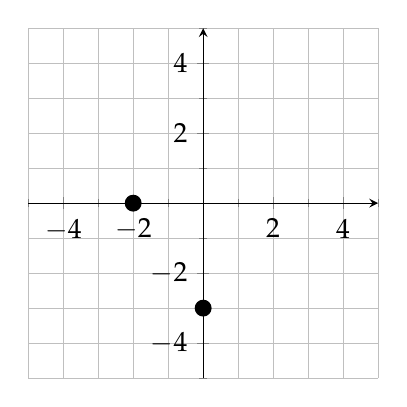
\begin{tikzpicture}
            \begin{axis}[
                width=2.75in,
                grid=both,
                axis x line = middle,axis y line = middle,
                axis equal image,
                xtick distance = 2, ytick distance = 2,
                xmin = -5, xmax = 5,
                ymin = -5, ymax = 5,
                minor tick num = 1,
                ]
                \addplot[
                    only marks,
                    mark=*,
                    mark size = 0.1cm,
                    ] coordinates { (0,-3) (-2,0) };
            \end{axis}
        \end{tikzpicture}
    \end{center}
}{2.5in}

\myExample{
    Sketch the graph of the line with 
    \begin{itemize}
        \item $x$-intercept at (3,0)
        \item $y$-intercept at (0,4)
    \end{itemize}
}{3.25in}

% ---------------------LESSON 2------------------------------
\begin{myLesson}[][2]
    You already know how to sketch the graph
    of a linear equation in \emph{slope--intercept} form.
    You learned that in Algebra 1.
    These examples will remind you how it's done.
\end{myLesson}

% ---------------------CONCEPT 2------------------------------
\begin{myKeyConcepts}[To sketch the graph of a linear equation in slope--intercept form, $y=mx+b$\dots]
    Follow these steps:
    \setlist{labelindent=\parindent,}
    \begin{enumerate}
        \item {\bfseries\itshape Plot} the $y$-intercept point at $(0,b)$ on the $y$-axis. 
        \item {\bfseries\itshape Plot} more points using ``rise over run'' from the slope, $m$.
        \item {\bfseries\itshape Connect} the points with a straight line.
    \end{enumerate}
\end{myKeyConcepts}

\myExample{
    Sketch the graph of the following linear equation.
    \[
        y = x + 3 
    \]   
}{2in}

\myExample{
    Sketch the graph of the following linear equation.
    \[
        y = -3x + 2 
    \]   
}{2.5in}

\myExample{
    Sketch the graph of the following linear equation.
    \[
        y = \frac{1}{2}x -3
    \]   
}{2in}

\myExample{
    Sketch the graph of the following linear equation.
    \[
        y = -\frac{2}{3}x - 1
    \]   
}{2in}

To sketch the graph of any linear equation
(no matter what form it is in),
the main challenge is to convert it to slope--intercept form.
You learned this in Algebra 1.
These examples will remind you how to do it.

% ---------------------CONCEPT 3------------------------------
\begin{myKeyConcepts}[To sketch the graph of any linear equation\dots]
    Follow these steps:
    \setlist{labelindent=\parindent,}
    \begin{enumerate}
        \item {\bfseries\itshape Collect} all the like terms.
        \item {\bfseries\itshape Convert} to slope-intercept form, $y = mx + b$. (Get $y$ by itself.)
        \item {\bfseries\itshape Plot} the $y$-intercept point at $(0,b)$ on the $y$-axis. 
        \item {\bfseries\itshape Plot} more points using ``rise over run'' from the slope, $m$.
        \item {\bfseries\itshape Connect} the points with a straight line.
    \end{enumerate}
\end{myKeyConcepts}

Those last three steps are the same as what we just did.

\myExample{
    Sketch the graph of the following linear equation.
    \[
        y + 3x = 2 
    \]   
}{3in}

\myExample{
    Sketch the graph of the following linear equation.
    \[
        4x + 2y = -6 
    \]   
}{3.5in}

\myExample{
    Sketch the graph of the following linear equation.
    \[
        3x = 7 + 2y
    \]   
}{4in}

% ---------------------LESSON 4------------------------------
\begin{myLesson}[][3]
    Many students get confused by the equations of vertical and horiztonal lines.
    They struggle sketching them.
    Remember,
    \begin{myLessonBox}
        {\bfseries\itshape Horizontal} lines run left and right.
        All the points on the line have the same $y$ coordinates.
        So the equation of a horizontal line looks like
        \[ y = k \]
        where $k$ is a constant number.
    \end{myLessonBox}
    \begin{myLessonBox}
        {\bfseries\itshape Vertical} lines run up and down.
        All the points on the line have the same $x$ coordinates.
        So the equation of a horizontal line looks like
        \[ x = h \]
        where $h$ is a constant number.
    \end{myLessonBox}
\end{myLesson}

By the way, the constants $h$ and $k$ can be positive or negative.
{\bfseries\itshape They can also be zero.}
For example, $x=0$ is the equation of a vertical line that goes through the origin.

% ---------------------CONCEPT 4------------------------------
\begin{myKeyConcepts}[To sketch horizontal and vertical lines\dots]
    For {\bfseries\itshape horizontal} lines, $y=k$, follow these steps.
    \setlist{labelindent=\parindent,}
    \begin{enumerate}
        \item {\bfseries\itshape Plot} a point on the $y$-axis at $(0,k)$.
        \item {\bfseries\itshape Draw} a horizontal line left and right from that point.
    \end{enumerate}
    \vspace{1em}
    For {\bfseries\itshape vertical} lines, $x=h$, follow these steps.
    \begin{enumerate}
        \item {\bfseries\itshape Plot} a point on the $x$-axis at $(h,0)$.
        \item {\bfseries\itshape Draw} a vertical line up and down from that point.
    \end{enumerate}
\end{myKeyConcepts}

\myExample{
    Sketch the graph of $x=3$.
}{2in}

\myExample{
    Sketch the graph of $x=-4$.
}{2in}

\myExample{
    Sketch the graph of $y=5$.
}{2in}

\myExample{
    Sketch the graph of $y=0$.
}{2in}

% \begin{myProblems2}%
%     {Factor the following monomials into prime factors.}%
%     {2in}%
%     %
%     {\( 32x^2 \)}
%     {\( 8 x^3y^2z \)}
% \end{myProblems2}
  


\end{document}